\listfiles
\documentclass[12pt]{article}
% -------------------------------------------------------------------
% Basic packages
\usepackage[english]{babel}
\usepackage[utf8]{inputenc}
\usepackage[T1]{fontenc}
\usepackage{lineno}
\usepackage{hyperref}
\usepackage{graphicx}
\usepackage{natbib}
\usepackage{fancyhdr}
\usepackage{setspace}

% -------------------------------------------------------------------
% Math packages
\usepackage{amsmath,amsfonts,amssymb,amsthm,cancel,siunitx,calculator,calc,mathtools,empheq,latexsym,inputenc}
% -------------------------------------------------------------------
% Packages for figures
\usepackage{subfig,epsfig,tikz,float}
% -------------------------------------------------------------------
% Packages for tables
\usepackage{booktabs,multicol,multirow,tabularx,array}

% -------------------------------------------------------------------

% Margins

\usepackage[a4paper,
            bindingoffset=0.2in,
            left=1in,
            right=1in,
            top=1.2in,
            bottom=1.2in,
            footskip=.25in]{geometry}

\linespread{2}
\linenumbers


% -------------------------------------------------------------------
% Title
\title{\renewcommand{\baselinestretch}{1.17}\large\bf The Foraging-mode Paradigm: A Historical Overview Including a Reevaluation of its Predictions
}

% -------------------------------------------------------------------
% Authors

% Authors
\author{\normalsize
Dylan J. Padilla Perez, John VandenBrooks, \& Michael J. Angilletta Jr.
}


% -------------------------------------------------------------------

% Begin document

\begin{document}

\date{}

\maketitle

\vspace{-0.5cm}

School of Life Sciences, Arizona State University, Tempe, Arizona 85287, USA. \vspace{6pt} \\ \textbf{Corresponding author:} dpadil10@asu.edu; \textbf{Phone:} +1 (480) 646-7769

\vspace{6pt}


% -------------------------------------------------------------------
% Abstract
%\bigskip
%\newpage
\noindent
{\normalsize{\bf Abstract}
\newline

}

\medskip
\noindent
{\small{\bf Keywords:}{ environmental heterogeneity, foraging gene, $G \times E$ interaction, life history.} 


}

\baselineskip=\normalbaselineskip
% -------------------------------------------------------------------

\newpage
\noindent
\section*{\normalsize Introduction}

A central tenet in behavioral ecology is to determine how organisms exploit food in a given environment \citep{macarthur1966optimal}. In nature, food is found in patches or lumps that vary in quality or density over time. In response to such environmental heterogeneity, organisms adopt certain foraging behaviors that maximize their fitness \citep{schoener1969models}. For instance, an active-foraging behavior is attributed to an organism that frequently abandons foraging sites. When the foraging site is rarely abandoned, the organism rather displays a sit-and-wait behavior. This behavioral dichotomy is currently known as ``The Foraging-mode Paradigm''; a categorization that may seem somewhat crude but most researchers would agree that many organisms fall clearly at the extremes of a continuum. A seemingly tireless hummingbird that visits flowers in search of nectar, as opposed to a kingfisher that waits on a perch and swoop in the water when a fish passes by, are perfect examples to illustrate this point.

\vspace{20px}

Since the early 1970s, researchers have developed mathematical models to specify which behavior is best suited for an organism to maximize energy intake in a particular environment, leading to the invention of the optimal foraging theory \citep{schoener1971theory,charnov1976optimal}. However, the initial application of the optimal foraging theory was to explain the evolution of body sizes of organisms with little emphasis on their foraging mode. This theory was later extended in models that explicitly compared between foraging modes as alternative strategies among species \citep[e.g.,][]{vitt1978body,janetos1982active}. Specifically, the models focused on investigating two main predictions: 1) Organisms should have a simple decision rule for giving up at a foraging site. They should move only when the expected gain from moving surpasses the expected gain from remaining at the foraging site. 2) If individual variation in foraging behavior affects the energetic benefits/costs, differences in growth rate, body size, and reproductive output are expected among individuals. This expectation is supported by the idea that different behavioral strategies determine the life histories of organisms by limiting their acquisition and allocation of energy to vital processes. An allocation tradeoff suggests that an increment in energy allocated to one function results in a decrement in energy allocated to other functions. Thus, an individual that acquire greater surplus energy may growth faster, have both a smaller body size and greater reproductive output \citep{stearns1992evolution,roff2002life}.

\vspace{20px}

Such predictions were instantly evaluated in a few elegant works fueled by the increasing interest in behavioral ecology at the time. The first empirical evidence derived from field studies of lizards \citep{vitt1978body,vitt1982ecological}. In a comparative analysis of reproductive output among species, the authors showed that active foragers had lower reproductive investment than did sit-and-wait foragers, with the rationale being that carrying a voluminous clutch while pursuing a prey increases the probability of being killed by a predator or reduces the foraging efficiency. Interestingly, a different study on orbweaver and sheetweb weaver spiders indicated that active foragers are subject to lower energetic costs \citep{janetos1982foraging}. Orbweavers seemed to evaluate whether to stay or leave the web based on the abundance of prey they capture in a day (i.e., the quality of the foraging site). As expected from active foragers, orbweavers leave the web in search of a better foraging site when the availability of prey is low. By contrast, sheetweb weavers seemed to be sit-and-wait predators, staying on the web for a longer time and only leaving it at random. Surprisingly, the author showed that sheetweb weavers pay a much higher energetic cost for constructing a new web from body reserves than do orbweavers. It is important to point out that the analyses described above might have been confounded by the phylogenetic relationships among species. However, interspecific studies at the time unavoidably suffered from such bias as the development of phylogenetic comparative methods was only available until 1985 with the foundational paper published by \cite{felsenstein1985phylogenies}.

\vspace{20px}

In parallel to the findings described above, some works on the behavioral polymorphism in freely foraging \textit{Drosophila melanogaster} led to the discovery of the foraging gene \citep[``\textit{for}'',][]{sokolowski1980foraging}. This pioneering study showed that individual larvae differed in how far they traveled while foraging. Accordingly, individuals could be classified into rover or sitter behavioral morphs, with rovers traveling significantly longer distances than sitters while on a feeding substrate. The discovery of the ``\textit{for}'' gene was particularly important because it paved the way for researchers to better understand the genetic basis of foraging behavior. For instance, early genetic analyses mapped the difference in foraging behavior to chromosome 2, with rover showing genetic dominance over sitter \citep{de1987heredity}. Later work also localized the ``\textit{for}'' gene to the cytological location 24A2–24A4 on the left arm of chromosome 2 \citep{de1989genetic}. The prevailing ecological perspective of foraging behavior at the time was then complemented with the increasing interest in the study of the genetic basis of such behavioral polymorphism.

\vspace{20px}

As more data became available, novel insights into the evolution of foraging behavior flourished in recent decades. With the advent of next-generation sequencing, for example, we now know that geographic and ecological factors are responsible for important genetic differences at ``\textit{for}'' across populations of \textit{D. melanogaster} \citep{padilla2024geographic}. We also know that an epigenetic regulator of the ``\textit{for}'' gene (the G9a methyltransferase) is responsible for rover–sitter differences in adult foraging behavior \citep{anreiter2017epigenetic}. Evidence from behavioral ecology studies have shown conflicting results though. While early studies suggest that active foragers have lower reproductive investment than do sit-and-wait foragers \citep{vitt1978body,vitt1982ecological}, more recent evidence show either no differences in the life history between the two behavioral strategies \citep{mesquita2016life}, or an opposite pattern to what most researchers have previously found. That is, there is an interaction between reproductive effort and body size such that active foragers have greater reproductive output than do sit-and-wait foragers at large body sizes \citep{padilla2022correlated}. Therefore, the expectation of differences in the life history between active foragers and sit-and-wait foragers requires further investigation.

\vspace{20px}

Importantly, the vast majority of the evidence described above come from interspecific studies, which enable one to make plausible inferences that can be evaluated at the intraspecific level. Given its well-known behavioral polymorphism, \textit{D. melanogaster} provides a good opportunity to further investigate long-standing predictions of the foraging-mode paradigm. Here, we aimed to evaluate two predictions: 1) The distance travel by active foragers (rovers) and sit-and-wait foragers (sitters) may be determined by the distribution of food in the environment. 2) If variation in foraging behavior affects the energetic benefits/costs, differences in the life history (e.g., growth rate) should be observed between the two behavioral strategies. Our results suggest that environmental heterogeneity alters the foraging behavior of individuals sufficiently enough to stimulate a faster growth when food is lumpy in the environment. However, growth rate seems to be the same between active foragers and sit-and-wait foragers regardless of the distribution of food in the environment.

\vspace{20px}

\section*{\normalsize Materials and Methods}%\label{sec:2}

\subsection*{\normalsize \textit{Fly strains}}

The rover ($for^r$) and sitter ($for^s$) strains used in the experiments have isogenized $for^r$ or $for^s$ 2nd chromosomes, sharing isogenized X and 3rd chromosomes from the rover B15 strain as described in \cite{bauer1985genetic} and \cite{sokolowski1980foraging}. We maintained the flies at 25\textdegree C, in a 12:12h light/dark cycle at 60\% relative humidity with lights on at 08:00h. We reared populations of flies in 8oz round-bottom Drosophila bottles, with a standard yeast-sugar-agar medium as suggested by \cite{anreiter2016foraging}. Before the beginning of the experiments, we transferred the flies into holding empty bottles and capped them with grape plates containing a small amount of dry-active yeast to stimulate reproduction. We removed the grape plates from the bottles 22 hr after they were set up and discarded all larvae from the seeded grape plates using a dissecting probe. We then incubated the eggs that remained in the grape plates for 4 hr in standard conditions as described earlier. After 4 hr, we picked L1 larvae per strain from the grape plates and placed them on food plates (i.e., yeast-sugar-agar medium). Lastly, we collected the testing larvae (L3) about 10 hr before wandering, which generally corresponds to 72-96 hr after hatching \citep{anreiter2016foraging}.

\vspace{20px}

\subsection*{\normalsize \textit{Experimental design for prediction 1: Distance traveled by active foragers and sit-and-wait foragers}}

We measured the distance traveled by L3 larvae while foraging in two types of environments that differed in the distribution of food. While one environment consisted of yeast paste distributed in patches on Drosophila agar medium, the other one contained only a lump of the paste on the medium. We set up these environments in $32 \times 10$ mm petri dishes. To make the patchy environment, we used a $12ml$ insulin syringe to pour small drops of dry-active yeast mixed with water at a 1:2 ratio (weight to volume). We followed the same procedure to make the lumpy environment, but this time we poured the paste in such a way that a lump formed at the center of the plates (see supporting material for details). Importantly, the consistency of the paste, the volume used ($2\mu l$), and the configuration of the food were the same among the test plates (see supporting material for details). 

\vspace{20px}

We collected individual L3 larvae and placed them in the test plates for 1 hr period necessary for acclimatization. To do this, we first randomized the strain, the type of environment, and the position on the plates where the larvae were released. To randomize these factors, we used the ``\textit{sample}'' function available in the free software R v.4.3.2 \citep[2023-10-31,][]{rcore}, which enabled us to pick a sample of a specified size ($n=1$ in this case) from a vector of predefined elements (e.g., a vector of two characters: ``rover'' and ``sitter''). To run the experiments, we placed the plates in an incubator set up at 25\textdegree C and 60\% relative humidity. We then recorded the larvae for 30 min, using a camera held 30 cm above the plates. In each trial, we recorded four plates simultaneously as indicated by Figure S\ref{fig:1}. The experiments yielded a sample size of 106 larvae; 58 of which were tested in a patchy environment ($n=27$ rover, $n=31$ sitter), and 51 tested in a lumpy environment ($n=29$ rover, $n=22$ sitter). After the end of the experiments, all of the larvae were transferred back to food plates where they continued to develop.

\vspace{20px}

\subsection*{\normalsize \textit{Experimental design for prediction 2: Growth rate of active foragers and sit-and-wait foragers}}

To measure growth rate, we let L3 larvae develop in two different environments with food distributed in patches and lumps, as described earlier. We measured growth rate as the difference between the initial mass and the final mass of the larvae over a 24 hr period. To record the initial mass, we gently washed the larvae with 1-2 ml of water and dabbed them dry with a paper towel to avoid any confounding factor when weighing the larvae. We then weighed the larvae using a micro-analytical balance (Metler Toledo Model XPR6UD5), and transferred them into the test plates. The test plates were placed in an incubator set up at 25\textdegree C and 60\% relative humidity. After 24 hr, we weighed and recorded the final mass of the larvae following the same procedure described above. This experiment yielded a sample size of ...

\vspace{20px}

\subsection*{\normalsize \textit{Data analysis}}

The experiments performed to evaluate the predictions of this study corresponded to a $2^2$ factorial design. This particular design is referred to as a $2^2$ (read ``two-by-two'') factorial design because it combines two independent variables, each of which has two levels. For instance, fly strain can be viewed as a factor with two levels: ``rover'' and ``sitter''. Likewise,  the type of environment can also be encoded as a factor with two levels: ``patchy'' and ``lumpy''. Factorial designs are a simple, yet elegant, way of comparing the main effects of multiple independent variables and exploring possible interaction effects.

\vspace{20px}

Based on the notation used in this full factorial design, the two-way ANOVA model represents the most appropriate model to analyze the data. Accordingly, we fitted two ANOVA models as follows: 1) The first model described the effects of the strain and the environment on the distance traveled by the larvae. As mentioned earlier, we used a camera to record the movement patterns of the larvae. To analyze the recordings, we used the free software AnimalTA v.2.2.1 \citep{chiara2023animalta}; a video-tracking software that enabled us to analyze numerous videos recorded under the same conditions. 2) The second model described the effects of the strain and the type of environment on the growth rate of the larvae. In both models we not only tested the main effects, but also the interactions between the independent variables. To do so, we used the function ``\textit{lm}'' available in the free software R v.4.3.2 \citep[2023-10-31,][]{rcore}. To evaluate the models’ goodness of fit, we considered the adjusted $R^2$ of the models, which indicates the percentage of variance that the models could explain given the data. To produce a good visualization of our results and ensure that they are fully reproducible, we carried out all the analyses in the free software for statistical computing R v.4.3.2 \citep[2023-10-31,][]{rcore}.

\vspace{20px}


\section*{\normalsize Results}


\vspace{20px}


%\vspace{20px}

%\begin{singlespace}
%\noindent
%\textbf{Figure \ref{fig:1}.} 
%\end{singlespace}
%\vspace{20px}


%\vspace{20px}

%\begin{singlespace}
%\noindent
%\textbf{Figure \ref{fig:2}.} 
%\end{singlespace}
%\vspace{20px}

%\vspace{20px}

%\begin{singlespace}
%\noindent
%\textbf{Figure \ref{fig:3}.} 
%\end{singlespace}
%\vspace{20px}

\vspace{20px}


\section*{\normalsize Discussion}


\vspace{20px}


\vspace{20px}

\section*{\normalsize Acknowledgements}

\section*{\normalsize Data Accessibility Statement}%\label{sec:3}

A fully reproducible workflow of the data analyses, including R scripts and additional supporting material, is available in the following repositories: Github \url{}.

\section*{\normalsize Conflict of interest}%\label{sec:3}

The authors have declared no competing interests.

\section*{\normalsize Author Contributions}

Dylan Padilla: Conceptualization, data curation, and formal analysis. Writing – original  draft, writing –  review and editing. The authors agreed to be held accountable for the work performed herein.

\begin{singlespace}

% End of document
% -----------------------------
%\bibliographystyle{apalike} % Reference style
\bibliographystyle{apalike}
\bibliography{references} % List of references

\end{singlespace}

\newpage

\begin{singlespace}

\section*{\normalsize Tables with captions}

% latex table generated in R 4.3.2 by xtable 1.8-4 package
% Wed Jun 12 16:34:54 2024
\begin{table}[ht]
\centering
\caption{Caption here...} 
\begin{tabular}{lllll}
  \hline
 & Estimate & Std. Error & t value & Pr($>$$|$t$|$) \\ 
  \hline
(Intercept) & 3.22e-04 & 3.00e-05 & 1.07e+01 & 1.37e-18 \\ 
  strainSitter & 1.52e-05 & 4.57e-05 & 3.33e-01 & 7.40e-01 \\ 
  envPatchy & -1.66e-04 & 4.32e-05 & -3.83e+00 & 2.18e-04*** \\ 
  strainSitter:envPatchy & 3.13e-05 & 6.24e-05 & 5.01e-01 & 6.18e-01 \\ 
   \hline
\end{tabular}
\label{tab:2}
\end{table}
\newpage

\section*{\normalsize Figures with captions}

\begin{figure}[!htb]
%\centering
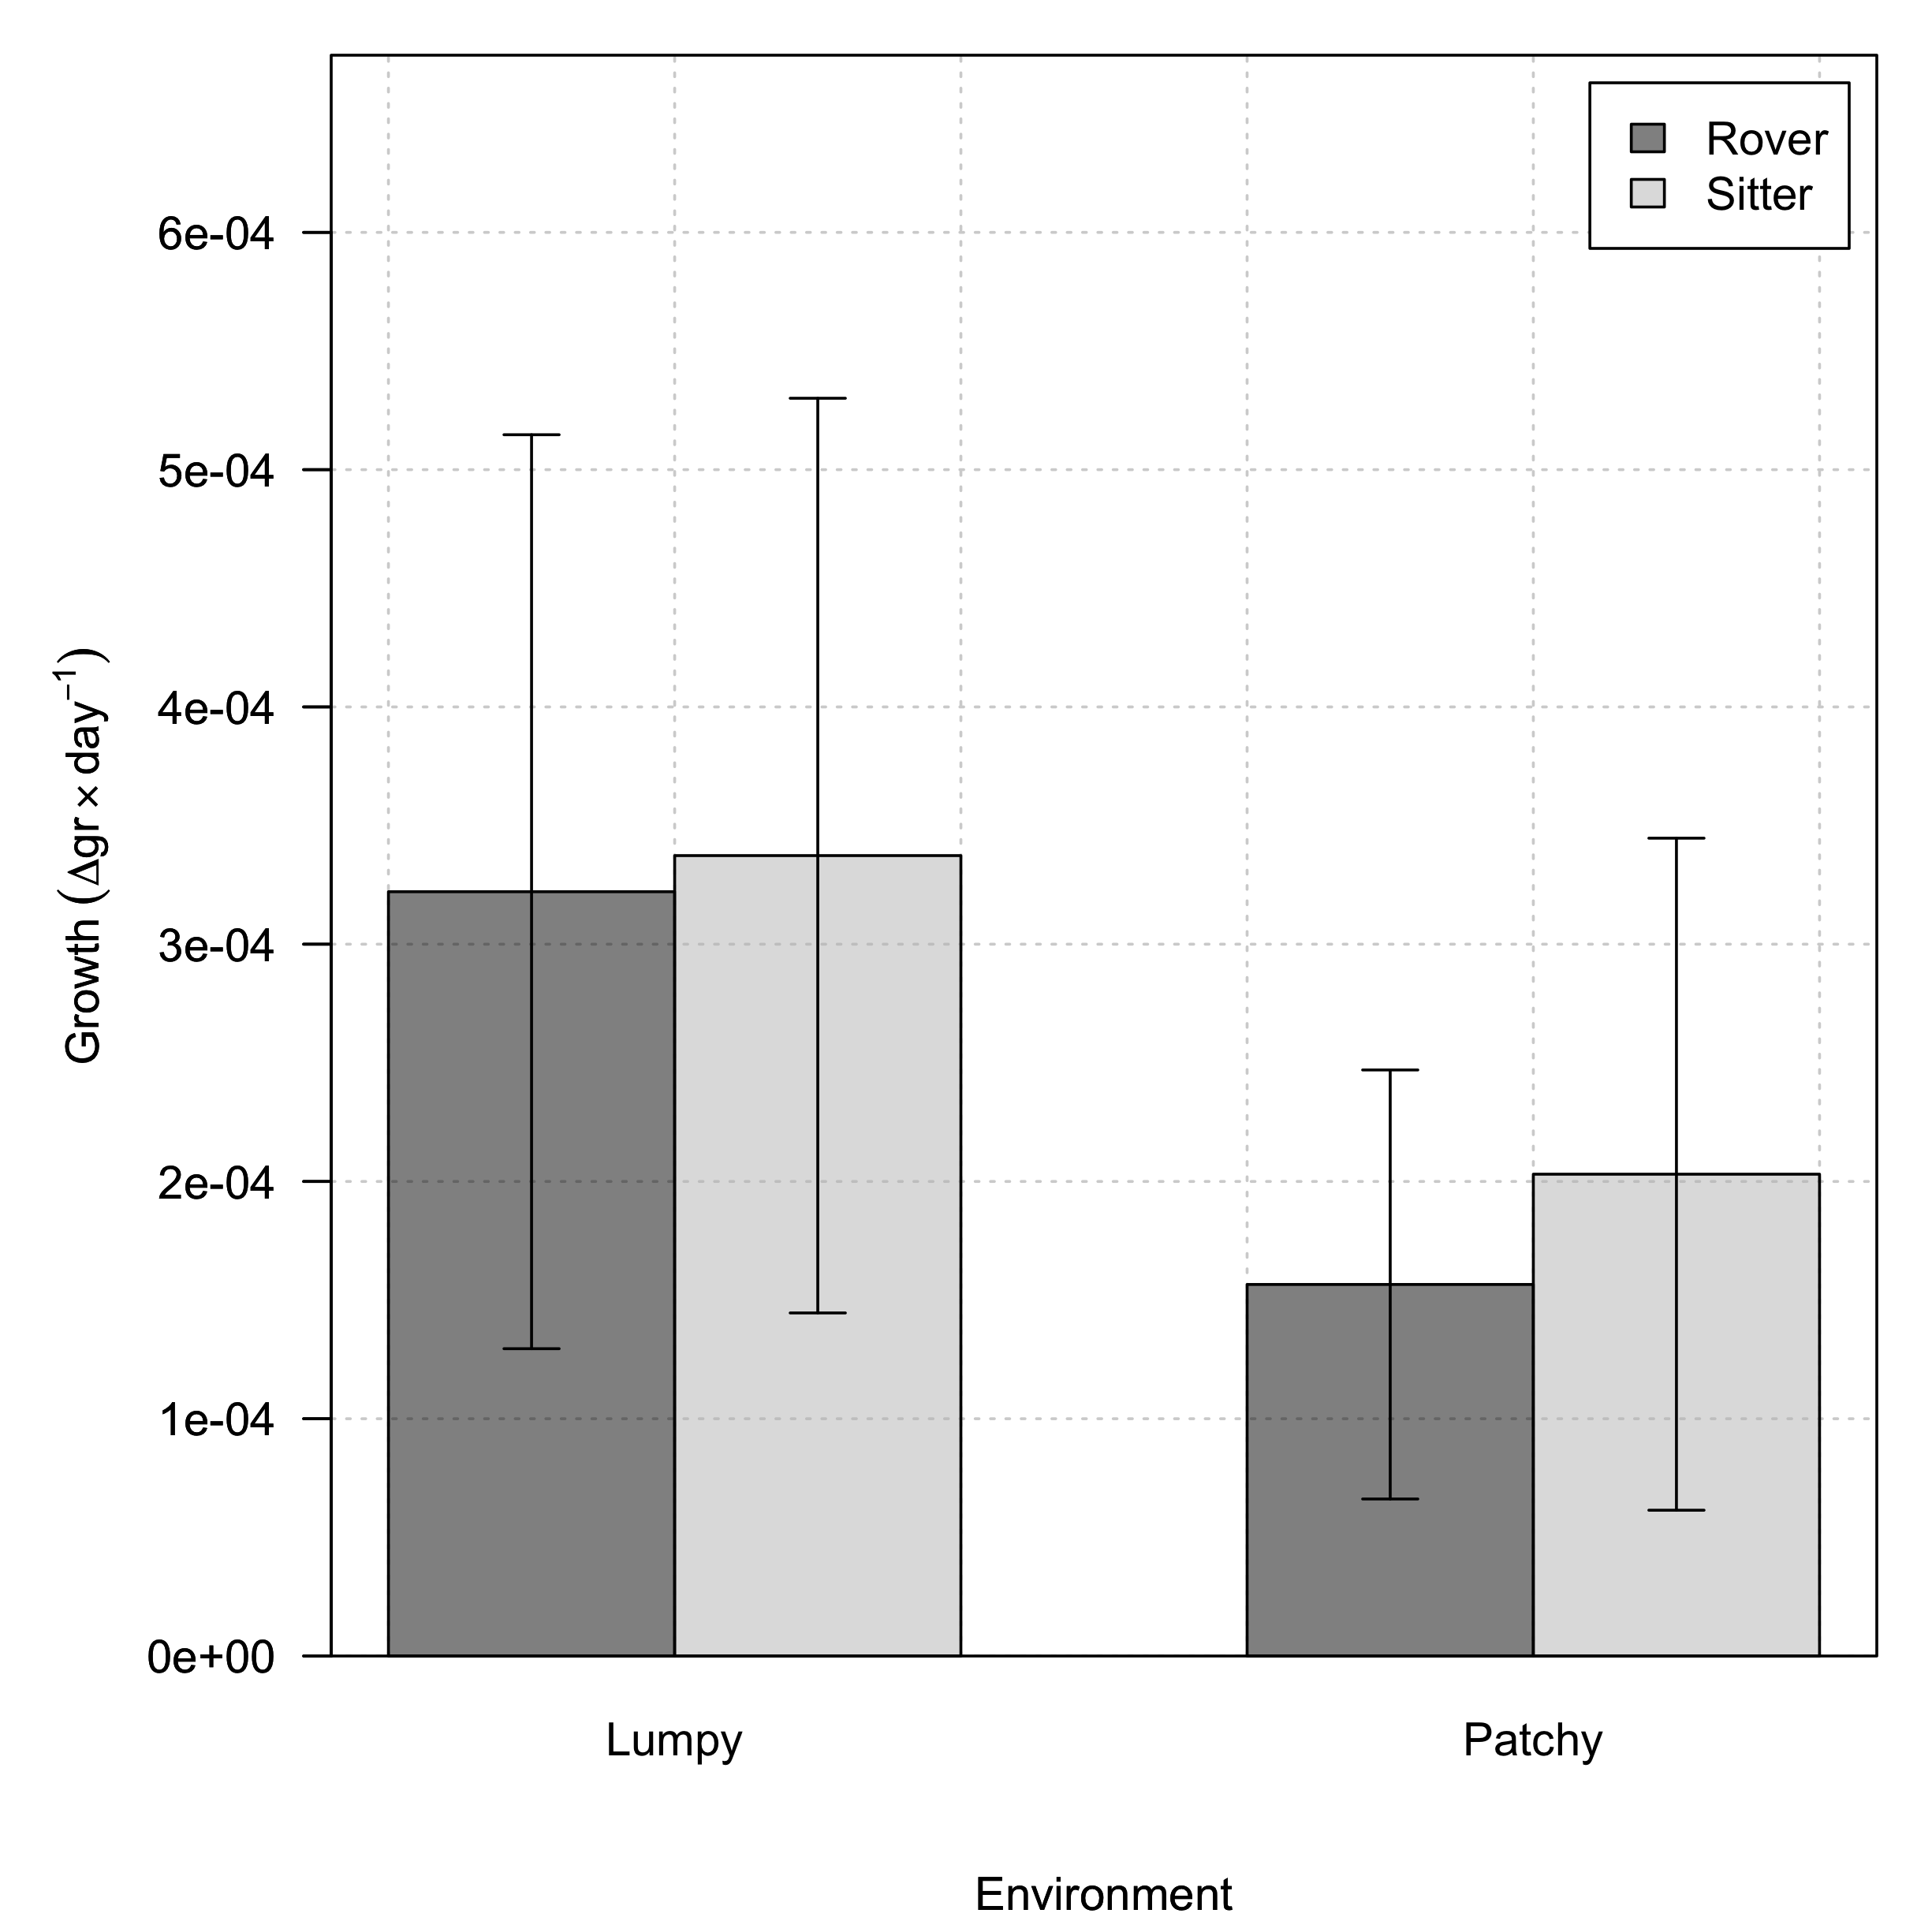
\includegraphics[scale=0.20]{imgs/figure2.png}
\caption{Caption here...}
\label{fig:2}
\end{figure}

%\newpage


%\begin{figure}[!htb]
%\centering
%\includegraphics[scale=1.2]{fig1.eps}
%\includegraphics[scale=0.20]{ }
%\caption{ .}
%\label{fig:2}
%\end{figure}

%\newpage

%\begin{figure}[!htb]
%\centering
%\includegraphics[scale=1.2]{fig1.eps}
%\includegraphics[scale=0.20]{ }
%\caption{ .}
%\label{fig:3}
%\end{figure}

%\newpage


\end{singlespace}

%\newpage

%\begin{singlespace}

%\section*{\normalsize Supplementary material}



%\end{singlespace}

\end{document}
